\documentclass[conference]{IEEEtran}
\usepackage{float}

% \IEEEoverridecommandlockouts
% The preceding line is only needed to identify funding in the first footnote. If that is unneeded, please comment it out.
\usepackage{cite}
\usepackage{amsmath,amssymb,amsfonts}
\usepackage{algorithmic}
\usepackage{amsmath}
\usepackage{graphicx}
\usepackage{textcomp}
\usepackage{xcolor}
\def\BibTeX{{\rm B\kern-.05em{\sc i\kern-.025em b}\kern-.08em
    T\kern-.1667em\lower.7ex\hbox{E}\kern-.125emX}}
\begin{document}

\title{Project Report: Interactive Car Game Using Microcontroller\\}

\author{
\centering
\IEEEauthorblockN{1\textsuperscript{st} Mateo Ronflard}
\IEEEauthorblockA{\textit{Computer Engineering} \\
\textit{McGill University} \\
Montreal, Canada \\
mateo.ronflard@mail.mcgill.ca, 260974012}
\vspace{1em}
\IEEEauthorblockN{2\textsuperscript{nd} Elie-Dimitri Abdo}
\IEEEauthorblockA{\textit{Computer Engineering} \\
\textit{McGill University} \\
Montreal, Canada \\
elie-dimitri.abdo@mail.mcgill.ca, 260948346}
\and
\IEEEauthorblockN{3\textsuperscript{rd} Alex Cattani}
\IEEEauthorblockA{\textit{Computer Engineering} \\
\textit{McGill University} \\
Montreal, Canada \\
alex.cattani@mail.mcgill.ca, 260924860}
\vspace{1em}
\IEEEauthorblockN{4\textsuperscript{th} Philippe Olivier Fils}
\IEEEauthorblockA{\textit{Computer Engineering} \\
\textit{McGill University} \\
Montreal, Canada \\
philippe.fils@mail.mcgill.ca, 260989600}
}
\maketitle

\begin{abstract}
This project implements a dynamic and interactive car game on an embedded system, showcasing advanced features such as UART communication for real-time game display, I2C-based tilt control for player interaction, auditory feedback through a DAC and speaker, and a custom operating system for thread management. The primary focus is on tilt control, which leverages accelerometer data to navigate menus and control car movements in the game. The mathematical principles behind tilt calculation, including angle determination and boundary constraints, are detailed. This project highlights the integration of hardware and software to achieve a responsive and engaging gaming experience, demonstrating the capabilities of microcontroller-based systems in real-time applications.
\end{abstract}

\textbf{Keywords:} Embedded systems, UART communication, tilt control, DAC, real-time operating system, interactive gaming, accelerometer, I2C, thread management.

\section{Introduction}
Embedded systems have revolutionized the way we interact with technology, enabling the creation of sophisticated real-time applications with minimal hardware. This project focuses on the design and implementation of an interactive car game using an embedded microcontroller. By leveraging advanced communication protocols, audio-visual feedback mechanisms, and multitasking capabilities, this game demonstrates the potential of embedded systems in delivering engaging user experiences.

The game consists of multiple interconnected features, including real-time game display via UART, tilt-based controls using I2C, auditory feedback through a DAC and speaker, and a custom operating system (OS) for managing threads. These features collectively form a robust system that highlights the importance of integrating software and hardware for high-performance embedded applications.

Tilt-based control is the core feature of this project, offering an innovative way for players to navigate menus and control the car's movement during gameplay. The accelerometer data is processed using mathematical models to calculate the tilt angle and translate it into meaningful actions. This ensures an intuitive and responsive user interaction, bridging the gap between physical movements and in-game actions.

By detailing both the design and implementation, this report aims to showcase not only the technical accomplishments but also the methodologies used to achieve a seamless gaming experience. The project demonstrates the versatility of embedded systems in creating real-time interactive applications, making it a valuable learning experience and a proof of concept for future developments.

\section{Project Features}
\subsection{UART Communication for Game Display}
The game leverages UART communication to print the road layout and car position on a terminal. This feature provides real-time visual feedback of the car's movement relative to the road boundaries. The dynamic display updates continuously as the player interacts with the game, making it easy to monitor gameplay progress. This feature highlights the integration of serial communication protocols to achieve seamless data transfer.

\subsection{Tilt Control Using I2C}
The tilt control feature is central to the game, allowing the player to navigate the car within the game environment and interact with the menu. This functionality is achieved by interfacing an accelerometer with the microcontroller via the I2C protocol. The accelerometer measures the tilt angles of the device, which are used to determine the car's movement and menu selections.

\subsubsection{Mathematics Behind Tilt Control}
The accelerometer provides raw data in three axes: $x$, $y$, and $z$. These values are processed to calculate the tilt angle $\theta$, which determines the car's movement. The tilt angle can be calculated using the following formula:
\begin{equation}
\theta = \arctan\left(\frac{y}{z}\right),
\end{equation}
where $y$ and $z$ are the accelerometer readings along their respective axes.

To map the tilt angle to car movement, we define thresholds for left and right turns. For example:
\begin{align}
\text{Left Turn:} & \quad \theta > \theta_{\text{threshold}}^{+}, \\
\text{Right Turn:} & \quad \theta < \theta_{\text{threshold}}^{-}.
\end{align}

The car moves straight when $\theta$ is within a neutral range:
\begin{equation}
\theta_{\text{threshold}}^{-} \leq \theta \leq \theta_{\text{threshold}}^{+}.
\end{equation}

These thresholds are calibrated based on gameplay requirements, ensuring responsiveness and accuracy.

\subsubsection{Menu Navigation Using Tilt Control}
Tilt control is also used for menu navigation. The accelerometer readings are processed similarly, with predefined tilt ranges mapped to menu options. For example:
\begin{align}
\text{Option 1:} & \quad \theta < \theta_{\text{menu}}^{-}, \\
\text{Option 2:} & \quad \theta_{\text{menu}}^{-} \leq \theta \leq \theta_{\text{menu}}^{+}, \\
\text{Option 3:} & \quad \theta > \theta_{\text{menu}}^{+}.
\end{align}

This intuitive control mechanism enhances user experience and eliminates the need for additional buttons or input devices.

\subsection{Auditory Feedback Using DAC and Speaker}
Auditory feedback is provided through a speaker connected to the microcontroller's DAC. This feature generates sound effects when the car interacts with the game environment, such as collisions, crossing boundaries, or successfully completing a level. The DAC converts digital signals into analog waveforms, driving the speaker to produce sound. This enhances the game’s interactivity by engaging multiple senses.

\subsubsection{Speaker Setup}
The speaker is connected to the DAC output pin on the microcontroller. The DAC is configured to produce varying signal levels to modulate sound pitches and volumes. Key details include:
\begin{itemize}
    \item \textbf{Hardware Connection:} The DAC output is connected to a low-power speaker via a coupling capacitor to filter out DC offsets.
    \item \textbf{Signal Modulation:} The DAC generates waveforms of different frequencies and durations to create distinct sound effects.
    \item \textbf{Volume Control:} By adjusting the amplitude of the generated waveform, the volume can be controlled programmatically.
    \item \textbf{Improved Loudness:} The speaker's volume was optimized by ensuring maximum safe DAC output levels and experimenting with different coupling capacitor values to enhance audio output.
\end{itemize}

\subsubsection{Sound Effects Implementation}
The game features multiple sound effects to enhance player immersion:
\begin{itemize}
    \item \textbf{Collision Alert:} A sharp tone of fixed duration to notify the player of a collision.
    \item \textbf{Boundary Warning:} A short beep when the car attempts to cross the road boundaries.
    \item \textbf{Victory Sound:} A sequence of tones of varying pitches and durations to celebrate reaching the finish line.
    \item \textbf{Game Over Sound:} A descending sequence of tones to signal the end of the game after a collision.
\end{itemize}
The sounds are generated using sine wave approximations at specific frequencies and durations. These parameters were fine-tuned to ensure clarity and distinguishability.

\subsection{Operating System for Thread Management}
An operating system is implemented to manage threads for various tasks, including input handling, game logic, display updates, and sound generation. The OS ensures efficient multitasking and real-time responsiveness, critical for an interactive game. Key functionalities include:
\begin{itemize}
    \item \textbf{Task Scheduling:} Allocating CPU time to different tasks based on priority.
    \item \textbf{Synchronization:} Preventing resource conflicts among threads.
    \item \textbf{Resource Management:} Efficiently handling shared resources like memory and peripherals.
\end{itemize}

\section{Game Features}
The interactive car game is designed to provide an engaging and immersive experience by simulating a car navigating a road with obstacles. The game incorporates a variety of features to ensure challenging gameplay and responsive mechanics. This section outlines the core aspects of the game, including obstacle generation, collision detection, boundary enforcement, and finish-line checking.

\subsection{Overview of the Game}
The player controls a car navigating through a dynamically generated road. The road is displayed on a terminal via UART, providing real-time feedback on the car's position relative to road boundaries and obstacles. The car is moved using tilt-based controls, where the player tilts the device to steer left or right. The objective is to safely navigate the road, avoid obstacles, and reach the finish line.
\subsection{Game Menu}
The game menu was designed to let the player decide the difficulty of the game each time the game is reset.

\subsubsection{Game Menu Functionality}
The game menu is displayed to the player whenever the game is first launched or after the player has won or lost a game. It lets the player select the different level difficulty: easy, medium and hard. As seen in Figure \ref{fig:game_menu}, the menu consists of a movable arrow and the selectable difficulties. The player can move the arrow to choose which level they want to play by tilting the board, the same way they would move the car once in play. Once the player's decision is made, they click on the blue button of the board to launch the game with the selected difficulty level. 
\begin{figure}
    \centering
    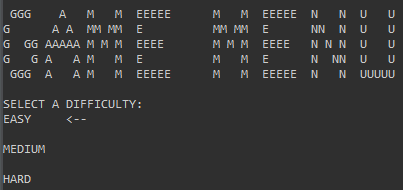
\includegraphics[width=1\linewidth]{game_menu.png}
    \caption{Game Menu displayed on the Terminal}
    \label{fig:game_menu}
\end{figure}

\subsubsection{Implementation of the Game Menu}
In order to make sure that the transition between the game menu and the actual game is done correctly, the OS task responsible for the game behavior and display is suspended as soon as the program is launched. The game menu task is set to high priority and will then be launched. A mutex is used to lock the resources used to read the accelerometer and process the board's tilt to avoid the other threads using them simultaneously. 

The difficulty of the game is set based on the position of the game menu arrow. If the arrow is at position 0, the difficulty is easy. If the arrow is at position 1, the difficulty is medium and if the arrow is at position 2, the difficulty is hard. It also sets where the arrow should be displayed in the menu. The difficulty level of the game determines how many obstacles will be generated.

When the player is ready to play and presses the start button, the game parameters such as the position of the car and the state of the game board are reset, the game difficulty is set, and the task in charge of the game behavior is resumed. This allows the game to start in its initial state. The game menu task is also suspended. It will only be resumed once the player loses or wins the game.

\subsection{Obstacle Generation}
Obstacles are placed randomly along the road to create a challenging environment for the player. The generation algorithm ensures that:
\begin{itemize}
    \item Obstacles are positioned within the road boundaries.
    \item The spacing between obstacles varies, maintaining unpredictability.
    \item No two obstacles overlap, ensuring clear paths for the player to navigate.
\end{itemize}
A pseudo-random number generator is used to determine the obstacle positions, with parameters tuned to balance difficulty and fairness.

\subsection{Collision Detection}
Collision detection is a critical feature to determine whether the car hits an obstacle. This is achieved by comparing the car's position to the positions of all obstacles within the same row on the terminal display. Mathematically, if the car's coordinates $(x_c, y_c)$ match an obstacle's coordinates $(x_o, y_o)$, a collision is detected:
\begin{equation}
\text{Collision: } (x_c = x_o) \land (y_c = y_o)
\end{equation}
When a collision is detected, an alert is triggered, and auditory feedback is provided through the speaker using the DAC.

\subsection{Boundary Enforcement}
To ensure that the car remains within the road boundaries, the system constantly checks its position against the road limits. The road boundaries are defined as the minimum and maximum permissible $x$-coordinates:
\begin{equation}
x_{\text{min}} \leq x_c \leq x_{\text{max}}
\end{equation}
If the car attempts to move beyond these boundaries, the movement is restricted, and a warning sound is played to notify the player.

\subsection{Finish Line Detection}
The finish line is positioned at the end of the road and serves as the game's endpoint. When the car reaches the finish line's $y$-coordinate:
\begin{equation}
y_c = y_{\text{finish}}
\end{equation}
a victory message is displayed on the terminal, and a celebratory sound is generated through the speaker. This marks the successful completion of the game.

\subsection{Integration of Features}
These features are seamlessly integrated to deliver a cohesive gameplay experience. The system ensures real-time updates to the terminal display and accurate feedback to the player, making the game intuitive and engaging. Each feature contributes to the overall challenge and enjoyment, highlighting the capabilities of the embedded system.

\section{Conclusion}
This project demonstrates a range of microcontroller capabilities through an interactive car game. The ambitious features, particularly tilt control, showcase advanced interfacing, mathematical processing, and intuitive user interaction. The combination of UART communication, auditory feedback, and multitasking through an operating system further highlights the project’s complexity and innovation. The code is structured and well-documented to ensure readability and maintainability.

\end{document}
